\subsection{Muon spectrometer}

Muon spectrometer is the outermost part of the ATLAS detector with an extremely large tracking system.
It measures a large range of muon momentum, and the accuracy can be about 3\% at 100 GeV and 10\% at 1 TeV.
The muon spectrometer is comprised of three main parts: a magnetic field produced by three toroidal magnets;
a set of chambers measuring the tracks of muons with high spatial precision; and triggering chambers with accurate time-resolution. 
Figure~\ref{fig:muon_dec} shows the schematic of ATLAS muon spectrometer, from which you can see four types of muon chambers as well as the magnet systems (barrel and end-cap toroid).
\begin{figure}[!htb]
  \centering
  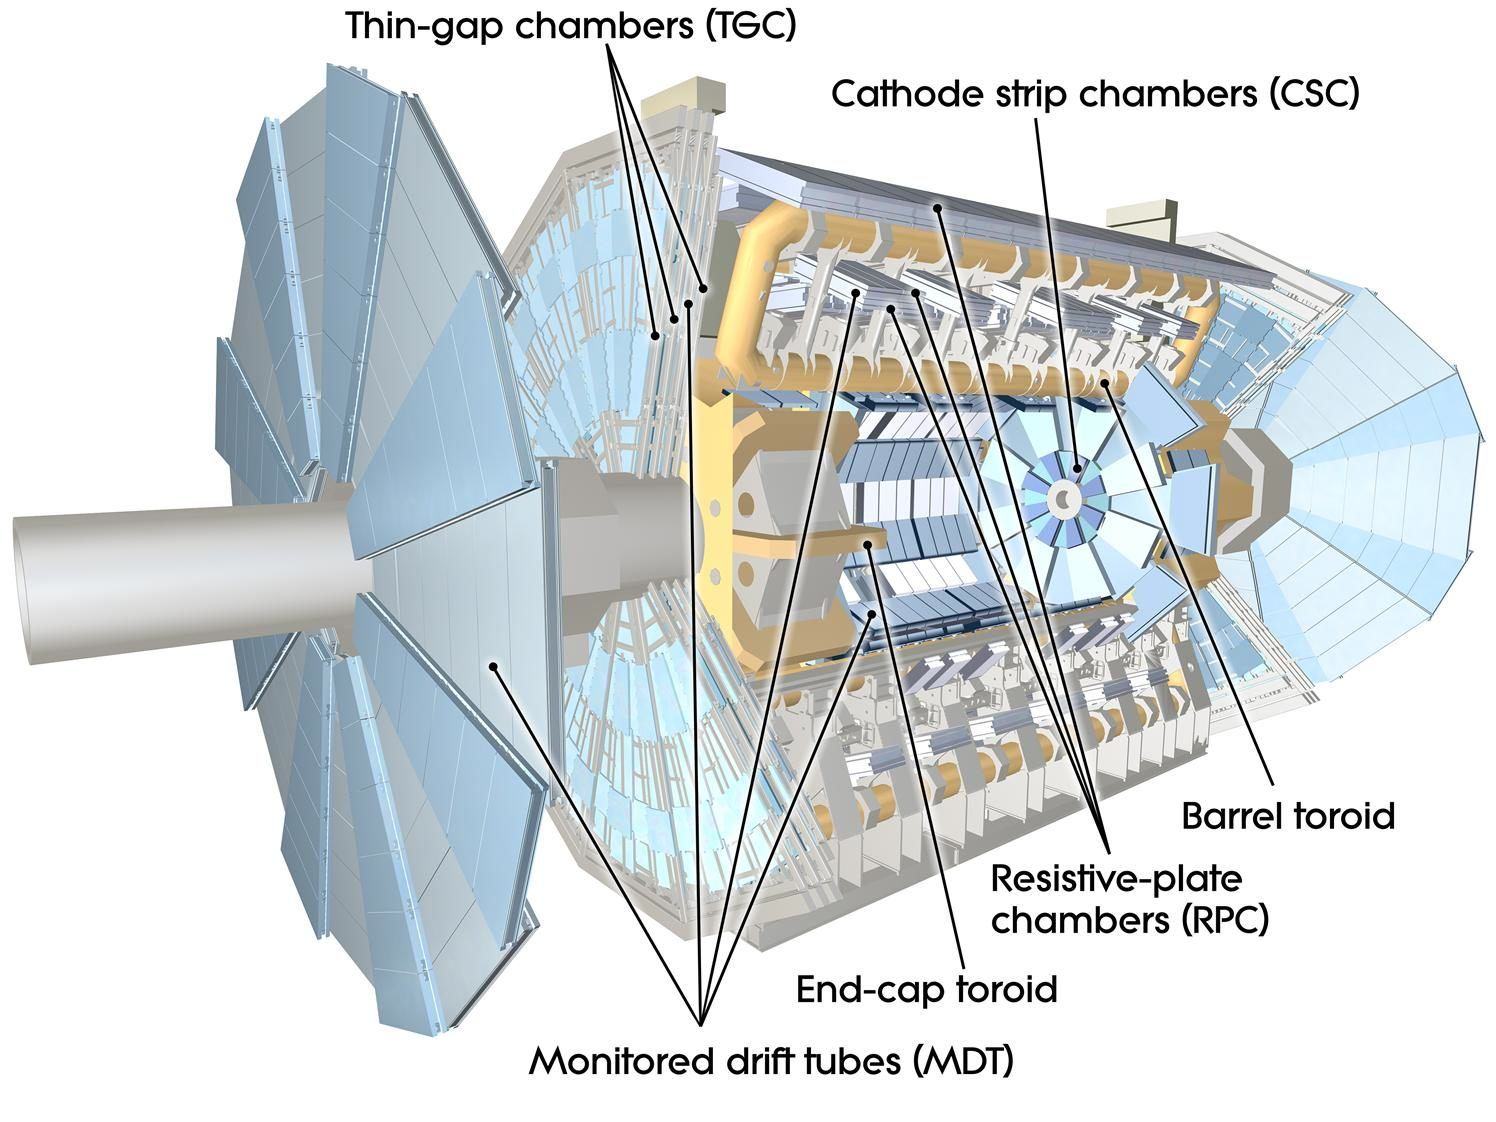
\includegraphics[width=0.9\textwidth]{figures/Detector/muon_all.png}
  \caption{Cut-away view of the ATLAS muon spectrometer\cite{Sliwa:2013oua}.}
  \label{fig:muon_dec}
\end{figure}
The details of four-type chambers are given as belows:
